\section{Introduction}\label{s:intro}
Distributed and cloud computing applications require the endpoint network stack to provide more than just (reliable or unreliable) communication channels accessed via the sockets API.
Many applications 
instead use higher-level communication primitives such as remote procedure calls (RPCs)~\cite{birrell1984implementing} and publish-subscribe (pub/sub)~\cite{virtual-synchrony} communication. 
To perform well and meet their service-level objectives (SLOs), applications need low latency and/or high throughput from these libraries. 

Operating systems and shared libraries have evolved so that it is simpler to write networked applications that implement complex logic and meet stringent performance requirements. For example, new kernel network interfaces such as io\_uring~\cite{iouring} and kernel bypass libraries such as DPDK~\cite{dpdk} reduce software overheads and improve communication performance.
Further, RPC libraries such as gRPC~\cite{grpc} and Thrift~\cite{thrift} and communication services such as Kafka~\cite{kafka} and Google PubSub~\cite{gcp-pubsub} implement useful communication primitives. 
Meanwhile, in modern deployments, several network functions are often packaged into higher-layer (\ie application-facing) middleware libraries (\eg ServiceRouter~\cite{service-router}) or ``sidecar proxies'' such as Envoy~\cite{envoy} and Istio~\cite{istio}.

The problem, however, is that these communication libraries often make {\em deployment assumptions} to implement their functionality or meet performance requirements.
For example, kernel bypass libraries (and io\_uring under some settings) achieve low latency by requiring that each application thread be ``affinitized'' to a CPU core that is not shared with other threads or processes, thus limiting what other applications the host can run.
Similarly, most pub/sub libraries rely on an external pub/sub service, 
imposing additional overheads if the application is deployed outside the corresponding cloud provider's datacenter.

While libraries that make deployment assumptions have become necessary for application performance and efficiency, their use
also constrains the application \emph{administrator's} choices, since changing resource allocations or deploying in a different environment can require significant changes to application code. 
For example, reconfiguring a kernel-bypass application to allow sharing application cores with other applications would require changing its code to use a different I/O abstraction (\eg sockets) or switching from polling to interrupt-driven I/O. 
Even when deployed in the same location, an administrator might want to change an application's libraries to cope with changes in workload.
For example, an administrator might want applications to use different pub/sub services (with different cost and scalability trade-offs) depending on the number of subscribers.

For these reasons, when choosing communication libraries, application developers must consider not only application requirements but also possible deployment locations and workloads.
Accounting for all of these factors, however, is complicated and nearly impossible. Thus, developers today must choose between specialized and performant libraries that limit where an application is deployed and how it responds to workload changes and general libraries that provide flexibility but with poorer performance and fewer features.

To resolve this tradeoff, this paper presents \name,
a network stack that allows developers to use specialized communication libraries and interfaces that make deployment assumptions but enable those decisions to be reconfigured both when deploying an application and at runtime. 
\name does so by allowing application developers to specify several alternate implementations of the same functionality and providing mechanisms to switch between these alternatives at runtime.

\name's core enabling abstraction is the {\em \tunnel}.
A \tunnel, similar to a library, implements some communication functionality, \eg for kernel-bypass networking, serialization, and pub/sub communication.
A developer can implement the \tunnel trait (or interface) to expose some functionality to a \name application.
Applications can \emph{compose} a sequence of \tunnels when creating a connection (Figure~\ref{f:chunnel-basic}).
We use the term ``\tunnel stack'' to refer to the sequence of \tunnels available for a connection; all data sent or received over the connection is processed in sequence by \tunnels in the stack.
Developers specify reconfiguration choices by specifying multiple \tunnels (or a composition of \tunnels) at a particular layer of the stack: in this case, the \name runtime chooses one of these when making a connection and provides a mechanism for the application to change its choice later. We assume that the application can function correctly with any of these \tunnel choices. The only constraint \name imposes on alternate \tunnels in a layer is type safety (\S\ref{s:chunnel-impl}). 
Thus, alternate \tunnels in a layer can make different deployment assumptions and provide different performance and efficiency trade-offs,  allowing application developers to use feature-rich, high-performance communication libraries without limiting an administrator's ability to change deployment environments.

\begin{figure}
    \centering
    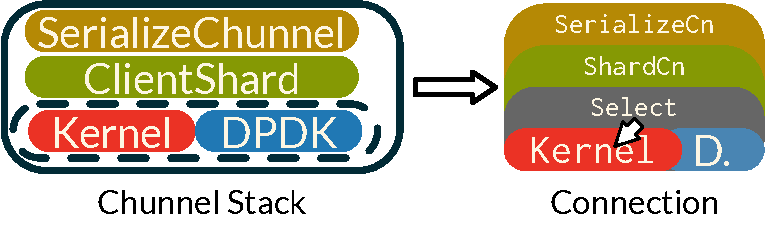
\includegraphics[width=\columnwidth]{img/chunnel-basic}
    \vspace{0pt}
    \caption{A \name connection specifies a \emph{\tunnel stack}, which composes multiple \tunnels. \tunnel stacks can express options (\eg here between Kernel and DPDK), and at runtime \name can create a connection using one set of options (here, Kernel) and also \emph{reconfigure} this choice later (\S\ref{s:reconfig}).}
    \label{f:chunnel-basic}
\end{figure}

\tunnels enable reconfigurability and extensibility by providing:
\begin{inparaenum}[(a)]
    \item a uniform interface for receiving and sending data, ensuring that switching between different \tunnels does not require any changes to application code or logic;
     \item a typed interface, allowing \name to check during compilation that reconfiguration cannot change the type of input data (\eg bytes, strings, or objects) that a \tunnel processes, nor change the type of outputs it produces; and
     \item embedded runtime type information that allows \name to ensure compatibility between the \tunnels used by a connection's endpoints.
\end{inparaenum}

\paragrapha{Contribution.}  \name is the first network stack to support safe reconfiguration mechanisms for arbitrary communication libraries, through a combination of compile-time constraints (\S\ref{s:chunnel-impl}) and runtime checks (\S\ref{s:reconfig}).
Previous work (\S\ref{s:relwork}) has provided only point solutions for specific libraries.

In \S\ref{s:applications}, we evaluate the performance benefits \name can provide by safely enabling the use of optimized communication libraries with an example Extract, Transform, Load (ETL) application implemented with \name.
We find that \name 
can unlock application optimizations such as using client-side sharding to achieve $16\times$ higher load meeting a $50$ $\mu$s target latency for a sharded key-value store (\S\ref{s:app:lb}) or 63\% lower latency for a publish-subscribe benchmark (\S\ref{s:app:pubsub}).
Further, our evaluation in \S\ref{s:eval} shows that \name's abstractions that enable reconfigurability and extensibility add no overhead for most applications and only a 27\% throughput overhead in the worst case (for the highest-performance applications using minimum-sized packets).
